\chapter{Power law phenomenon}
\section{The power law}
Initially the simplest distribution assumed for the degree distribution on a social network is a \textit{Normal Gaussian}. But it is verified that the distribution of the degree is proportional to $ f(k) = \frac{1}{k^\beta} $ with $ \beta  $ close to 2. A function $ f(k) $ that decrease as increase $ k $ is called \textit{power law}
\subsection{Difference between a normal distribution and a power law}
The normal distribution is a representation of a balanced phenomenon, where in the mean there is the maximum frequency and in the slopes decrease the frequency.\\
In the power law instead is a representation of a imbalanced phenomenon where, with small values of x we have high frequency and with high values x we have a small frequency. Some example of power law phenomenon are the richness, number of relations in a social network.
\begin{figure}[H]
	\centering
	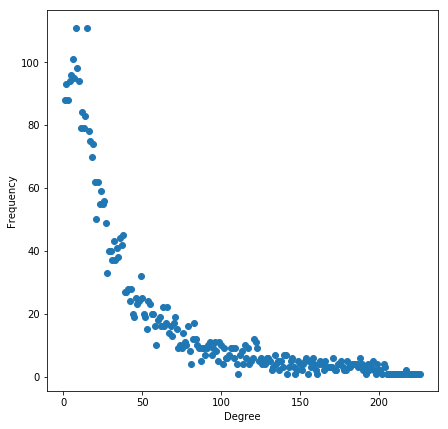
\includegraphics[width=0.7\linewidth]{img/power_law_example}
	\caption{Degree distribution on a Facebook social network}
	\label{fig:powerlawexample}
\end{figure}
\subsection{Check if a degree distribution is a power law}
In order to check if a degree distribution is a power law it must be in the form $ f(k) = \alpha \cdot \dfrac{1}{k^{\beta}} $.
We can do a linear regression in log-log scale of $ f(k) $ that is
\begin{align*}
\log(f(k)) = \log\left(\dfrac{\alpha}{k^{\beta}}\right) = \log(\alpha) - \beta \cdot \log(k)
\end{align*}
and should be a straight line to represent a power law

\section{Generative model of social network based on degree distributions}
In this section we study some generative models based on degree distribution of real graph. The generative models aim to estimate the $ p(x) $, the distribution of data that in this case is a social network
\subsection{Erd\"{o}s-Gilbert-R\'{e}nyi model}
This model is very simple, in fact it consider the probability \textit{p} that exists an edge between two nodes is independent to any other. \\ In statistical terms we can consider the distribution edge as a $ Bernoulli(k;p) $.\\ In this case we define the graph as $ G(n,p) $ where n is the number of nodes and p the probability that exists an edge.\\
The expected number of edges is:
%In prof handouts the formula is wrong, this is taken from https://economics.mit.edu/files/4621
\begin{align*}
\E \left[ Edges \right]= \sum_{1\leq x \leq y \leq n} (1\cdot p + 0 \cdot (1-p)) = \sum_{1\leq x \leq y \leq n} p = \binom{n}{2} p = \dfrac{n(n-1)}{2} p
\end{align*}
Since in a indirect graph an edge is present in the two extremes of the edge the expected degree of a node is $ 2 \cdot   \frac{n(n-1)}{2} p $.\\
The probability that a node have \textit{k} neighbours is a binomial distribution  so we can express as $ Bin(k; n, p) = \binom{n}{k} \cdot p^k \cdot (1-p) $. %also here an error on prof handouts 
\\
This model for \textit{n} and \textit{k} sufficiently big approximate to a normal distribution
\subsection{Chung-lu model}
In this model the probability that exists an edge between two nodes is proportional to the expected degree of the pair of nodes.
\begin{itemize}
	\item Initially we set $ \textbf{d} = (d_1 \ldots d_n) $, the expected degree of each node.
	\item The probability that exists an edge between the node \textit{i} and \textit{j} is \begin{align*}  p(E_{ij}) = \dfrac{d_i d_j}{\sum_k d_k} 	\end{align*} 
\end{itemize}
If the degree distribution \textbf{d} is a power law, then the graph generated is a power law
\subsection{Barabasi-Albert model}
The previous models are static, in fact they have a fixed number of nodes. \\This model is dynamic so it mean that doesn't require the number of nodes a priori but they can be added always.\\ 
With this dynamism try to give an explain to creation of a social network at difference of the previous models.\\
Every time a node is inserted an edge is created with the \textit{preferential attachment} system.
\subsubsection{Preferential attachment system}
Every time a node \textit{j} is added, a direct edge is created with the following two possibilities:
	\begin{itemize}
		\item with probability \textit{p} choose a random node $ i < j $  
		\item with probability $ (1-p) $ choose a node with probability proportional to the in-degree of the node
	\end{itemize}
The latter option is called \textit{rich-get-richer rule}. In fact if you have a  high number of relation you are more likely to make more.
\subsubsection{Degree distribution}
When a node \textit{j} is created, the probability that exists the edge $ (j, i)) $ with $ j > i $ is:
\begin{align*}
P(E_{ji}) &= \dfrac{1}{j-1} \cdot p + \dfrac{G_i(j-1)}{\sum_{h \leq (j-1)} G_h(j-1)} \cdot (1-p) \\
&=  \dfrac{1}{j-1} \cdot p + \dfrac{G_i(j-1)}{j-1} \cdot (1-p) 
\end{align*}
where $ G_i(j-1) $ is the in-degree of the node \textit{i} at the time $ j-1 $
\subsubsection{Deterministic $ G_j(t) $}
We want to find an approximation of $ G_j(t) $ that give deterministically the in-degree of a node $ l $ at time $ t $. Let us denote as $ g_l(t) $ the approximation of $ G_l(t) $. The increase of in-degree can be expressed from a differential equation:
\begin{align*}
	& \dfrac{d(g_l(t))}{dt} = \dfrac{p}{t} + \dfrac{ g_l(t) \cdot (1-p)}{t} = \dfrac{p + g_l(t) (1-p)}{t} \\
	& \dfrac{d(g_l(t))}{dt} \cdot \dfrac{1}{p + g_l(t) (1-p)} =  \dfrac{1}{t} \\
	& \int \dfrac{d(g_l(t))}{dt} \cdot \dfrac{1}{p + g_l(t) (1-p)} dt = \int   \dfrac{1}{t}  dt \\
	& g_l(t) \cdot \dfrac{\ln(p + g_l(t) (1-p))}{1-p} + c' = \ln(t) + c'' \\
	& g_l(t) \cdot  \ln(p + g_l(t) (1-p)) =  \ln(t) \cdot (1-p) + c \\
	& e^{\ln(p + g_l(t) (1-p))} = e^{\ln(t) \cdot (1-p) + c} \\
	&e^{\ln(p + g_l(t) (1-p))} = e^{\ln(t) \cdot (1-p) } \cdot e^c \\
	&(p + g_l(t) (1-p)) = t^{(1-p) } \cdot e^c \\
	& g_l(t) = \dfrac{t^{1-p} \cdot e^c - p}{1-p}	 
\end{align*}
When we insert the node $ l $ at time $ l $ we have that $ g_l(l) = 0  $ so we have
\begin{align*} 
 & 0= \dfrac{l^{1-p} \cdot e^c - p}{1-p}	 \\
 & \dfrac{p}{1-p} =\dfrac{l^{1-p} \cdot e^c}{1-p} \\
 &	e^c = \dfrac{p}{l^{1-p}}
\end{align*}
if we substitute the latter expression in $ g_l(t) $ we have
\begin{align*}
	 &g_l(t) = \dfrac{t^{1-p} \cdot \dfrac{p}{l^{1-p}} - p}{1-p}  \\
	 &g_l(t) = p \cdot \left( \left(\frac{t}{l}\right)^{(1-p)}  -1 \right) \cdot \dfrac{1}{1-p}
\end{align*}
\noindent
We can use the latter expression to estimate the number of nodes that at time \textit{t} have degree at least \textit{k}. So we write
\begin{align*}
	& \left( \left(\frac{t}{l}\right)^{(1-p)}  -1 \right) \cdot \dfrac{p}{1-p} \geq k \\\\
	&\text{Then we pone respect to l: } \\
	& \left(\frac{t}{l}\right)^{(1-p)} \geq k \cdot \dfrac{1-p}{p} + 1 \\
	& \frac{t}{l} \geq \left(k \cdot \dfrac{1-p}{p} + 1\right)^{\frac{1}{1-p}} 
	\end{align*}
Note that the next expression is the fraction of nodes at time \textit{t} that have at least in-degree \textit{k}:
\begin{align*}
	 & \frac{l}{t}\leq \left(k \cdot \dfrac{1-p}{p} + 1\right)^{-\frac{1}{1-p}} \\
	  & l \leq t \cdot \left(k\cdot \dfrac{1-p}{p} + 1\right)^{-\frac{1}{1-p}}
\end{align*}
To have the nodes that have \textit{exactly k in-degree} at \textit{time t} we must take the opposite of derivative (why?) of $  \left(k \cdot \dfrac{1-p}{p} + 1\right)^{-\frac{1}{1-p}} $ respect to k.\\ The result is 
\begin{center}
	$ \dfrac{1}{1-p} \left( k \dfrac{1-p}{p} + 1 \right)^{-\left(1 + \frac{1}{1-p}\right)} $
\end{center}
We can infer from the latter expression that the distribution of in-degree nodes is a power law with exponent $ \beta =  1 + \frac{1}{1-p}$.\\
From 
\begin{itemize}
	\item  when $ p \simeq 1 $ we exponent disappear then we tend to Erd\"{o}s-Gilbert-R\'{e}nyi model.
	\item when $ p \simeq 0 $ we apply almost ever the Preferential Attachment  System,  so the new nodes will more probably link to others with high in-degree, that is very similar to what happen with Chung-lu model.
	\item The distribution disappear when $ p \propto k^{-2} $ %Not understand how
%	in fact we have\\ $ \left( k \dfrac{1-k^{-2}}{k^{-2}} + 1 \right)^{-\dfrac{1-k^{-2}+1}{1-k^{-2}}}  = \left( k \dfrac{1-k^{-2} + k^{-2}}{k^{-2}} \right) ^ {\dfrac{k^{-2}-2}{1-k^{-2}}}= k^{3 \cdot \dfrac{k^{-2}-2}{1-k^{-2}}}$
\end{itemize}